%% USPSC-Cap3-Conclusao.tex
% ---
% Conclusão
% ---
\chapter{Conclusion}
\label{ch:conclusion}

This work introduced a distributed reinforcement learning framework tailored for high-frequency trading environments,
based on a shared parallel environment architecture and an asynchronous messaging backbone.
The proposed system addresses several persistent limitations in traditional distributed RL approaches
including communication overhead, data staleness, and the computational inefficiency arising from duplicated environment simulations.
By reconfiguring the standard multi-agent interaction model into a parallelized,
shared-environment setting, this framework allows more efficient use of compute resources while preserving---
if not enhancing---the statistical diversity of sampled trajectories.

\section{Results}
\label{sec:results}

Throughout the design and evaluation process, emphasis was placed on reducing the straggler problem extend improving training throughput.
The use of a brokerless ZeroMQ Router/Dealer communication layout enabled asynchronous, low-latency interactions between workers and the central learner.
This design reduced idle time in the learning loop and facilitated scalable coordination across heterogeneous agents operating at different speeds.

The experimental results validate several hypotheses that guided this design.
Notably, the architecture reduced average environment processing latency compared to replicated-environment setups,
while maintaining convergence properties of the learned policy under asynchronous V-trace updates.
The shared environment approach demonstrated favorable scaling characteristics in terms of training speed and memory usage.

% Table comparing average per-agent environment step latency in shared vs. replicated setups.
% Description: Table comparing average and variance of step processing time (in milliseconds) for N agents across shared vs. independent environments.
\begin{table}[h!]
    \centering
    \begin{tabular}{|c|c|c|c|}
        \hline
        \textbf{Operation} & \textbf{Distributed Policy Updates} & \textbf{Centralized Policy Update} \\
        \hline

        Act & \SI{35.142}{\milli\second} & \SI{3.113}{\milli\second} \\
        Step & \SI{40.554}{\milli\second} &\SI{47.984}{\milli\second} \\
        Reset & \SI{12.709}{\micro\second} & \SI{12.302}{\micro\second} \\
        \hline
    \end{tabular}
    \caption{Trainer time benchmarks for ten worker instances. All operations are the average time for 100 episodes taken for each operation per rollout.}
    \label{tab:benchmarks}
\end{table}

% PLACEHOLDER: Table comparing training wall time vs. performance for different architecture configurations.
% Description: Table comparing final episodic return and total training time for
% (1) single-threaded baseline, (2) replicated multi-agent, (3) shared environment multi-agent (ours).
% Include columns for sample throughput and wall-clock convergence time.
\begin{figure}[htbp]
    \begin{minipage}[t]{0.48\textwidth}
        \centering
        \includegraphics[width=\textwidth]{images/results/loss_episode}
        \caption{Average training loss over time for the shared environment architecture.}
        \label{fig:loss}
    \end{minipage}
    \hfill
    \begin{minipage}[t]{0.48\textwidth}
        \centering
        \includegraphics[width=\textwidth]{images/results/performance}
        \caption{Performance comparison of the shared environment for different numbers of shared environments.}
        \label{fig:performance}
    \end{minipage}
\end{figure}
Another important contribution of this work is the empirical demonstration that asynchronous environment dynamics
can retain stability for non-stationary simulators representative of financial market dynamics.
These dynamics, characterized by frequent regime shifts and exogenous shocks, are particularly prone to introducing non-Markovian effects that degrade learning performance.
The architecture’s ability to tolerate these conditions while maintaining learning efficiency highlights its applicability to real-world algorithmic trading systems.

% PLACEHOLDER: Graph showing convergence rate with and without V-trace under regime shifts.
% Description: Plot showing episode return over time for (1) V-trace enabled, (2) V-trace disabled, during training in a simulated market with predefined regime switches.

While the system achieves positive results when increasing shared environments, both in terms of latency and compute utilization,
it also poses a discussion on the trade-offs of shared LOB environments.
The shared environment increases contention on the simulation process, which can become a bottleneck under extremely high agent concurrency.
Additionally, managing consistent rollout recording and replay in this context requires careful attention to buffering and message timing.
These aspects open future directions for improvement, such as adaptive load balancing across simulation shards, environment step batching,
or model-based simulation acceleration.

\begin{figure}
    \centering
    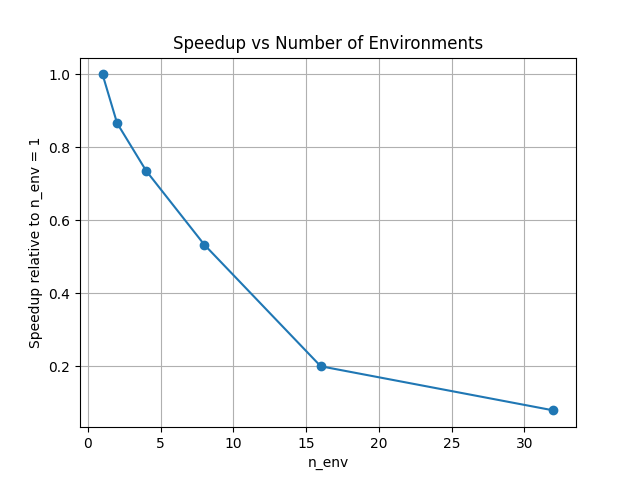
\includegraphics[width=0.6\textwidth]{images/results/speedup}
    \caption{Performance comparison of the shared environment for different numbers of shared environments.}
    \label{fig:speedup}
\end{figure}

\begin{table}[ht]
    \centering
    \begin{tabular}{|c|c|c|}
        \hline
        \textbf{Number of Environments} & \textbf{Loss per second (mean $\pm$ std)} & \textbf{wall time (mean $\pm$ std)} \\ \hline
        1  & 0.1408 $\pm$ 0.0661 & 205.03 $\pm$ 1.99 \\ \hline
        2  & 0.0923 $\pm$ 0.0082 & 236.32 $\pm$ 4.28 \\ \hline
        4  & 0.0696 $\pm$ 0.0042 & 278.28 $\pm$ 1.14 \\ \hline
        8  & 0.0452 $\pm$ 0.0025 & 382.98 $\pm$ 2.47 \\ \hline
        16 & 0.0166 $\pm$ 0.0010 & 1019.68 $\pm$ 5.35 \\ \hline
        32 & 0.0073 $\pm$ 0.0016 & 2591.26 $\pm$ 248.26 \\ \hline
    \end{tabular}
    \caption{Summary of Loss per Wall Time and Wall Time for Different n\_env Values}
    \label{tab:summary}
\end{table}


\section{Discussion}
\label{sec:discussion}

The modular nature of the framework facilitates integration with both existing financial simulators and real-time market data feeds.
The messaging and learner infrastructure are decoupled from environment specifics, enabling broader applicability beyond the specific HFT use case studied here.
In summary, this work contributes with:
\begin{itemize}
    \item An asynchronous architecture based on shared environments for distributed RL;
    \item A high-throughput, low-latency communication layer based on a brokerless messaging queue;
    \item Empirical evidence of improved convergence and latency profiles under real-time training constraints;
    \item Performance evaluation of a multi-agent, multi-environment market making policy under non-stationary, non-Markovian conditions.
\end{itemize}

The current PEARL architecture supports heterogeneous learners by allowing each instance to use a different algorithm
for each learner instance, so traders can test and train multiple different strategies together and independently.
Although fully developed, the architecture does not allow for strategies to communicate between each other,
and thus could be further extended to support Multi-policy learning (e.g., mixture-of-experts models).
Another promising area for future research is adaptive population scheduling—dynamically allocating computational resources to learners based on their performance.
Adaptative population scheduling can greatly reduce strategy exploration and exploitation costs,
thus enabling quantitative fund controllers adaptively prioritizing profitable strategies, especially in capital-constrained environments.

The results presented here demonstrate the feasibility and potential of designing systems that balance the algorithmic sophistication of
modern RL methods with the practical constraints and nature of high-frequency trading infrastructure.
The proposed framework provides a practical and scalable foundation for building high-performance simulators,
suitable for both academic research and real-time deployment in autonomous trading systems.
